
\documentclass[letterpaper, 11pt]{report}
\usepackage[utf8]{inputenc}
\usepackage{titlesec}
\usepackage{fullpage} % changes the margin
\usepackage{amsmath}
\usepackage{amssymb}
\usepackage{graphicx} %package to manage images
\usepackage[linkcolor=red]{hyperref}
\usepackage{paralist}
\usepackage{subcaption}
\graphicspath{ {./images/} }

\begin{document}
\begin{titlepage}
\vspace*{0.7in}
\begin{center}
\begin{figure}[htb]
\begin{center}

\includegraphics[width=8cm]{univ_logo}
\end{center}
\end{figure}
\vspace*{0.3in}
\begin{Large}
\textbf{SOEN 6011 : SOFTWARE ENGINEERING PROCESSES} \\
\end{Large}
\vspace*{0.1in}
\begin{Large}
\textbf{SUMMER 2021} \\
\end{Large}
\vspace*{0.9in}
\begin{Large}
\textbf{SUPER CALCULATOR} \\
\end{Large}
\vspace*{0.9in}
\begin{Large}
\textbf{PROBLEM - 1} \\
Function Description \\
\end{Large}
\vspace*{0.625in}
\rule{80mm}{0.1mm}\\
\vspace*{0.1in}
\begin{large}
Authors \\
\vspace*{0.1in}
Rokeya Begum Keya\\
\vspace*{0.1in}
Kyle Taylor Lange\\
\vspace*{0.1in}
Sijie Min\\
\vspace*{0.1in}
Manimaran Palani\\ 
\vspace*{0.3in}
\date{\normalsize\today} 
\end{large}
\end{center}
\begin{center}
https://www.overleaf.com/project/610304de4e6b8d24f7c781b6\end{center}
\end{titlepage}
\tableofcontents
\newpage
\addcontentsline{toc}{section}{a) Description of Functions}
\section*{Description of Functions}
\section*{\centering{PROBLEM 1 - F2: $tan(x)$}}
\normalsize {SOEN 6011 - Summer 2021} \hfill \textbf{Rokeya Begum Keya} \\
\textbf{ Software Engineering Processes}  \hfill \textbf{40183615} \\
\hfill Repository address : https://github.com/Dakatsu/SOEN6011Calculator
\\
 \subsection*{ Tangent Function, $tan(x)$ } 
 
 \normalsize{ \cite{test1} $tan(x)$ is a trigonometric function. There are many uses of tangent function for example, to find the slope of straight lines etc. By using the Unit circle, one can easily understand the tangent function. Moreover, in unit circle, one line is at the positive x-axis and the x coordinate intersects the circle is at $cos(x)$ and y coordinate intersects is at $sin(x)$. so, The tangent function is define as below: \[tan(x) = \frac{sin(x)}{cos(x)}\]
 }
 
 \subsection*{Graph}
 \begin{center}
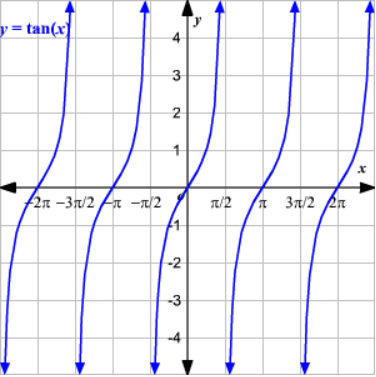
\includegraphics[width= 4cm]{tan}
\end{center}
\begin{center}
Graph of tangent function $ (tan(x))$\end{center}
 \normalsize{ \cite{test1} The tangent function is undefined when $x$ $=$ $\pi$ / 2 $+$ $n \pi$ (where, $n$ is integer) for which, $cos(x) = 0$. However, Tangent function does not have an amplitude. Inaddition, The graph intercept $x$-axis at $n\pi$ (where $n$ is integer) and in $y$-axis at $(0,0)$ point. The period of tangent function is $\pi$.
 }
 \\
 \subsection*{Range}
 \normalsize{ The range of $tan(x)$ is all real number $\mathbb{R}$, $(- \infty, + \infty)$. }
 
 \subsection*{Domain and Co-domain}
 \normalsize{The domain of tangent function is $x \in$ $\mathbb{R}$, $x$ $\neq$ $\pi$ / 2 $+$ $n \pi$ where, $n$ is an integer. The co-domain of $tan(x)$ is \((-\infty, +\infty\)).}
 
 
 \begin{thebibliography}{}
 
\bibitem{test1}
Malambo, Priestly. "Pre-Service Mathematics Teachers' Nature of Understanding of the Tangent Function." Journal of Research and Advances in Mathematics Education 5.2 (2020): 105-118.


\end{thebibliography}
 
 
 
 
\pagebreak

\section*{\centering{PROBLEM 1 - F3: Hyperbolic Sine, $sinh(x)$}}
\normalsize {SOEN 6011 - Summer 2021} \hfill \textbf{Kyle Taylor Lange} \\
\textbf{ Software Engineering Processes}  \hfill \textbf{27627696} \\
\hfill Repository address : https://github.com/Dakatsu/SOEN6011Calculator
\\\\\\\\\\
\normalsize{The function $sinh(x)$ is known as the hyperbolic sine, and it has the following formula \cite{sinh}. 
$$sinh(x) \equiv \frac{1}{2}(e^x-e^{-x})$$
The character $x$ is the only variable, as $e$ is a constant roughly equivalent to 2.71828 \cite{e}.

 \begin{figure}[SOEN_6011-Problem-1/images/desmos-graph-f3.png]
 \centering
 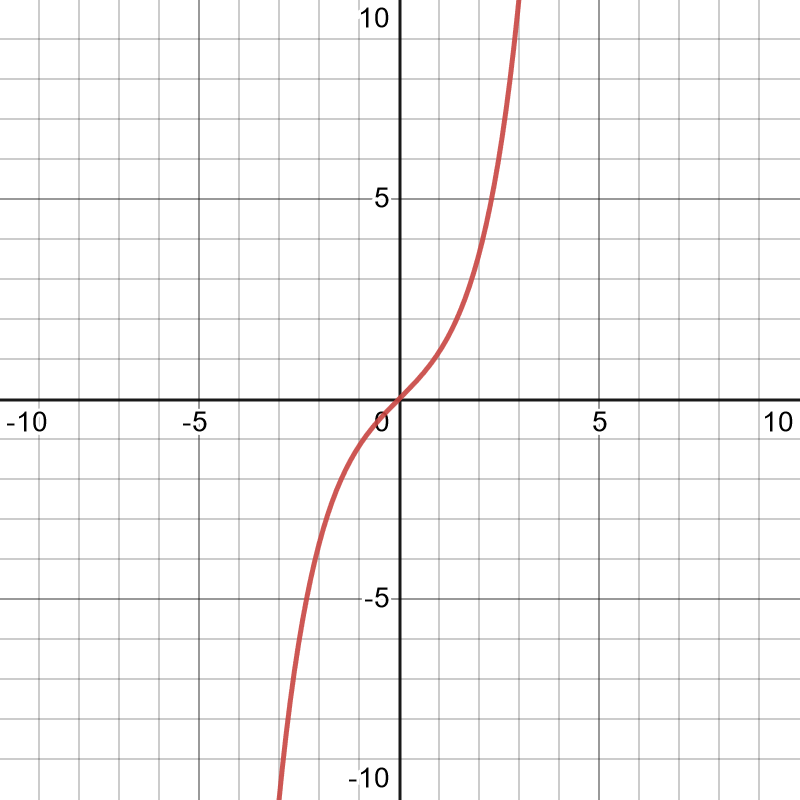
\includegraphics[width= 6cm]{SOEN_6011-Problem-1/images/desmos-graph-f3.png}
  \caption{A graph of $y = sinh(x)$ generated from Desmos.com}
\end{figure}

Both the domain and co-domain of $sinh(x)$ is $\mathbb{R}$, i.e. (-$\infty$, +$\infty$). Positive values of $x$ trend toward +$\infty$, negative values of $x$ trend toward -$\infty$, and an input of 0 outputs 0.
\\Just as the trigonometric functions sine and cosine relate to a unit circle \cite{circular}, their hyperbolic equivalents relate to the right branch of a unit hyperbola \cite{hyperbolic}. The x-coordinate of the right branch of the hyperbola at a given hyperbolic angle $a$ can be calculated with $cosh(a)$, and $sinh(a)$ will return the y-coordinate \cite{rectHyperbola}.}
\begin{thebibliography}{}
\bibitem{sinh}
Hyperbolic Sine, Wolfram MathWorld.
\\http://mathworld.wolfram.com/HyperbolicSine.html
\bibitem{hyperbolic}
Hyperbolic Functions, Wolfram MathWorld.
\\http://mathworld.wolfram.com/HyperbolicFunctions.html
\bibitem{circular}
Circular Functions, Wolfram MathWorld.
\\http://mathworld.wolfram.com/CircularFunctions.html
\bibitem{e}
e, Wolfram MathWorld.
\\http://mathworld.wolfram.com/e.html
\bibitem{rectHyperbola}
Rectangular Hyperbola, Wolfram MathWorld.
\\https://mathworld.wolfram.com/RectangularHyperbola.html
\end{thebibliography}
\pagebreak

\section*{\centering{PROBLEM 1 - F5}}
\normalsize {SOEN 6011 - Summer 2021} \hfill \textbf{Sijie Min} \\
\textbf{ Software Engineering Processes}  \hfill \textbf{401*****} \\
\hfill Repository address : https://github.com/Dakatsu/SOEN6011Calculator
\\\\\\
$y=a^x$ is called an exponential function, and it is one of the important basic elementary functions. For $y=ab^x$, a is a real number, $b^x$ is an exponential function, and a can be regarded as a scaling factor of the exponential function.
 \begin{center} 
\end{center}
\pagebreak

\newcommand{\R}{\mathbb{R}}
\renewcommand{\labelitemi}{$\star$}
\section*{\centering{PROBLEM 1 - F7 : \(x^y\)}}
\normalsize {SOEN 6011 - Summer 2021} \hfill \textbf{Manimaran Palani} \\
\textbf{ Software Engineering Processes}  \hfill \textbf{40167543} \\
\hfill Repository address : https://github.com/Dakatsu/SOEN6011Calculator
\subsection*{Definition of \(x^y\)}
\cite{mathInsight} Exponentiation is a mathematical operation, denoted as \(x^y\), If y is a positive integer and \(x\) is any real number, then \(x^y\) corresponds to repeated multiplication.
 \begin{center} \(x^y\) = \(x\)*\(x\)*\(x\)*.....*\(x\) of y times \end{center}
The expression can be called as “\(x\) raised to the power of y,” “\(x\) to the power of y,” or simply “\(x\) to the y.” Here, \(x\) is the base and y is the exponent or the power.
\subsection*{Domain}
\cite{mathbits} All the real numbers from -infinite to +infinite.(-\(\infty\) to \(\infty\))
 \begin{center} $(x,y) \in \R^2 : (x \geq 0 \land y \neq 0) \lor x>0$ \end{center}
\subsection*{Co-domain}
A set of all positive real numbers from zero to infinite (0 to \(\infty\)) is known as the Exponentiation function
\subsection*{Characteristics}
\begin{flushleft}
\textbf{Graph - }
 \end{flushleft}
\begin{flushleft}
\cite{mathbits}\cite{wolframalpha} The \textbf{rate of change} increases (or decreases) across the graph in an exponential graph.
\end{flushleft}
\begin{itemize}
\item \label{graph} The exponential graph crosses the y-axis at (0,1). 
\item The exponential graph increases, when x \(>\) 1.
\item The exponential graph decreases, when 0 \(<\) x \(<\) 1.
\item The exponential graph is asymptotic to the x-axis - gets very, very close to the x-axis but, in this case, does not touch it or cross it.
\end{itemize}
\begin{center}
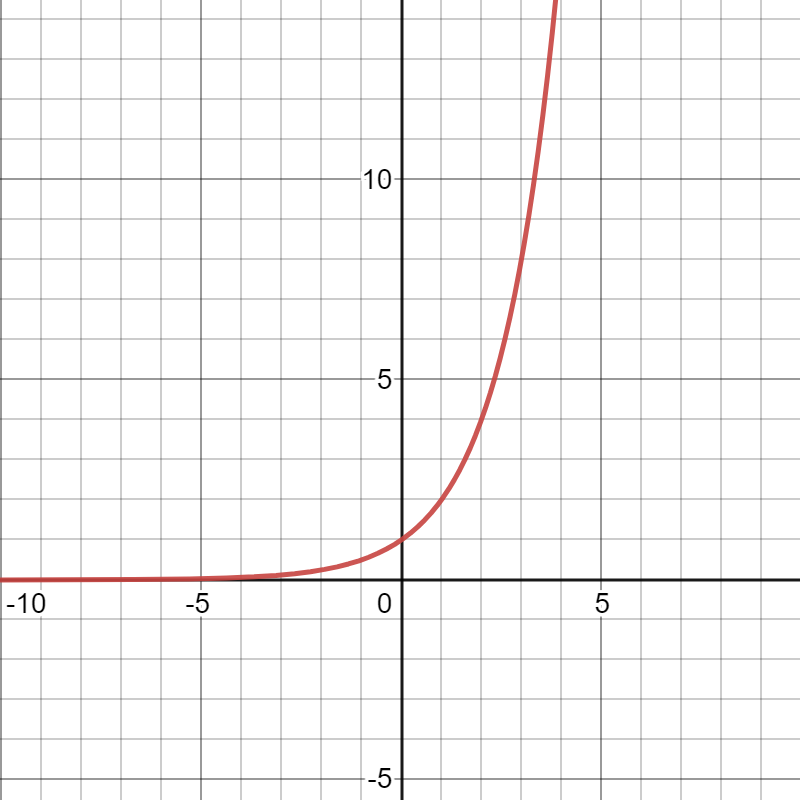
\includegraphics[width=5cm]{x^y}
\end{center}
\begin{center}
Graph crosses the y-axis at (0,1)\end{center}
\begin{thebibliography}{}
\bibitem{mathInsight} 
Nykamp DQ: Basic rules for exponentiation
\\\texttt{https://mathbitsnotebook.com/Algebra2/Exponential/EXExpFunctions.html}
\bibitem{mathbits} 
MathBits Teacher: Exponential Functions,
\\\texttt{https://mathbitsnotebook.com/Algebra2/Exponential/EXExpFunctions.html}
\bibitem{wolframalpha} 
WolframAlpha: Domain of exponentiation function,
\\\texttt{https://www.wolframalpha.com/input/?i=x\%5Ey}
\end{thebibliography}
\newpage
\addcontentsline{toc}{section}{b) Context of Use Model}I h
\section*{Context of Use Model}
\normalsize{The users of the calculator shall be using it to calculate the result of one of the four functions on a number. This number shall be an integer or decimal, so the digits \textit{0-9} and the decimal point must be enterable by the user. The user shall be able to select the appropriate function they wish to use, and they shall be able to press a key or button to indicate that they have finished inputting the number and wish to have the answer computed.}
\begin{center}
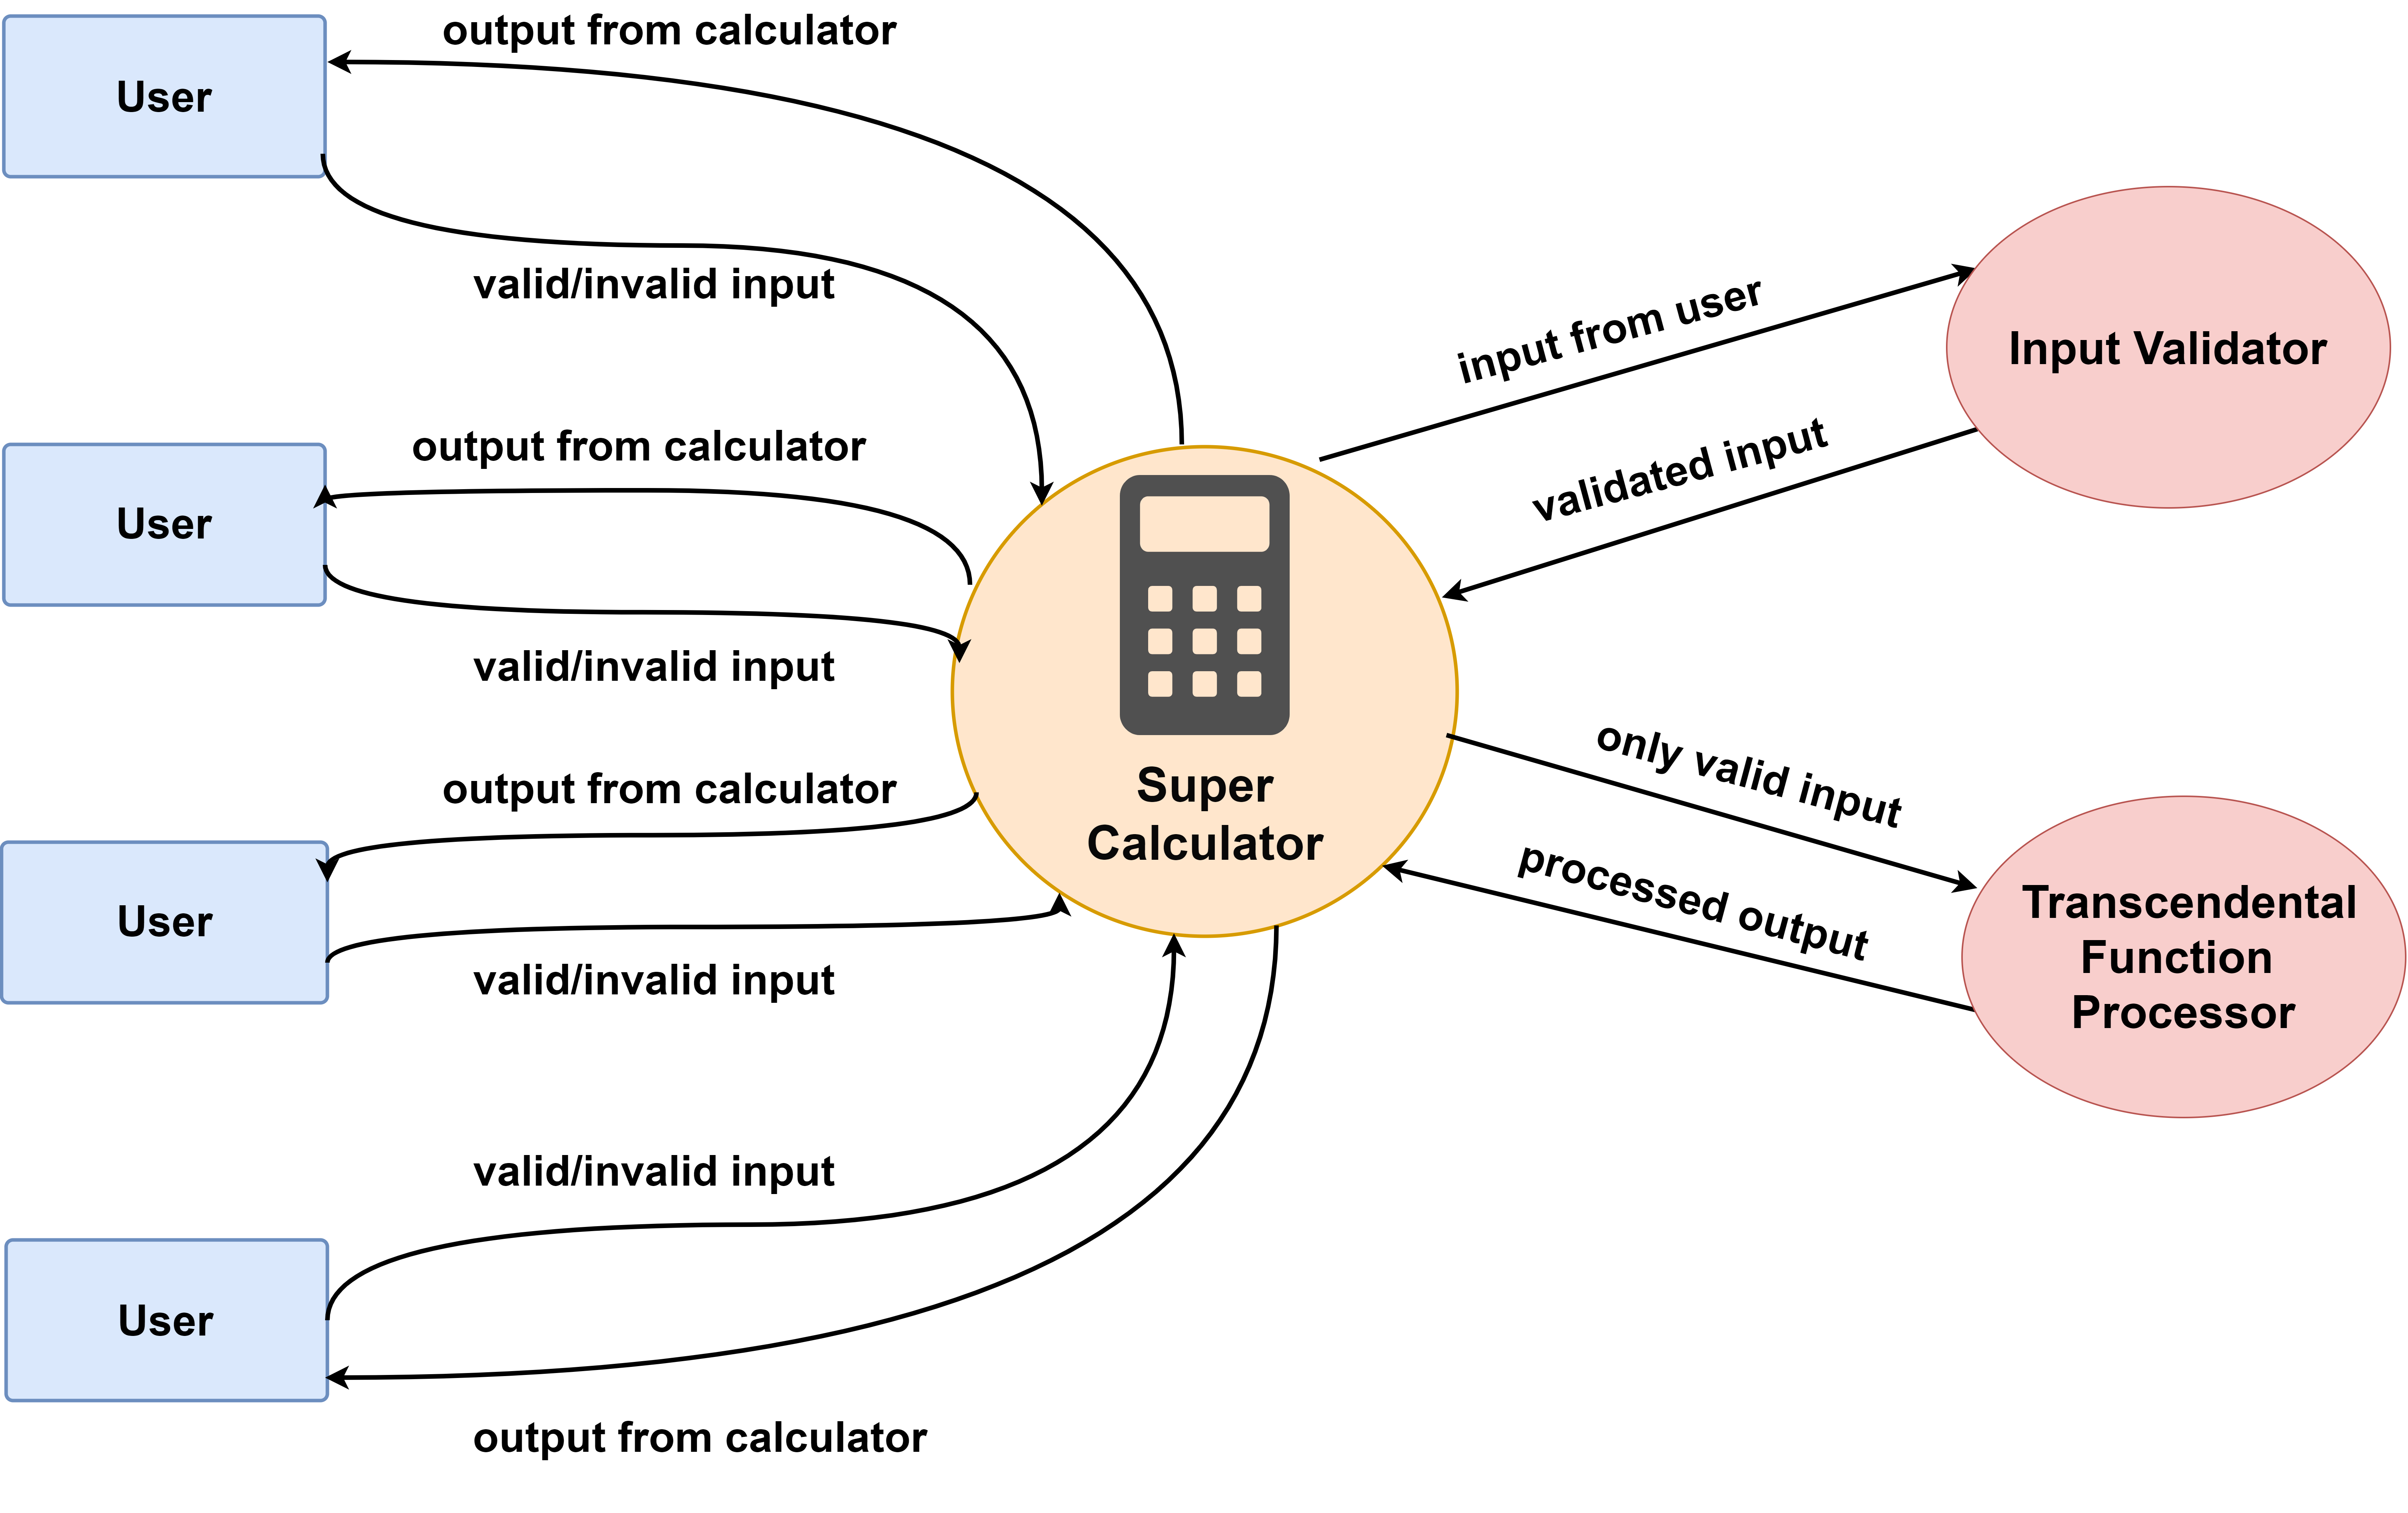
\includegraphics[width=15cm]{context_diagram}
\end{center}
\end{document}
